\documentclass[border=6pt]{standalone}
\usepackage{tikz}
\usetikzlibrary{arrows.meta,positioning,calc,shapes.geometric,fit,backgrounds,patterns,matrix,decorations.pathreplacing}
\begin{document}
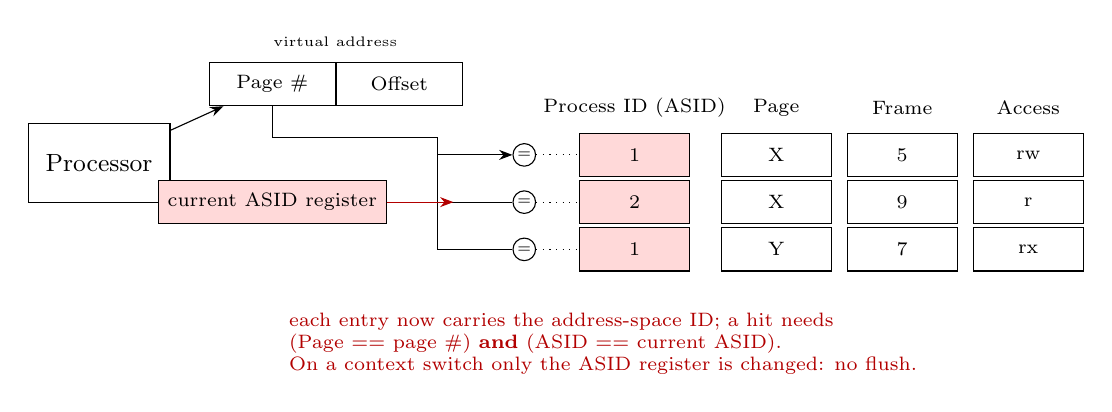
\begin{tikzpicture}[>=Stealth,font=\small]
\tikzstyle{c}=[draw,minimum height=0.55cm,font=\scriptsize]
\node[draw,minimum width=1.8cm,minimum height=1.0cm] (p) at (-5.2,0.8) {Processor};
\node[c,minimum width=1.6cm] (pg) at (-3,1.8) {Page \#};  \node[c,minimum width=1.6cm,right=0pt of pg] (of) {Offset};
\node[above=2pt of pg,xshift=0.8cm,font=\tiny]{virtual address};
\node[c,fill=red!15,minimum width=1.6cm] (cur) at (-3,0.3) {current ASID register};
\draw[->] (p) -- (pg);
\node[font=\scriptsize] at (1.6,1.5) {Process ID (ASID)};\node[font=\scriptsize] at (3.4,1.5) {Page};\node[font=\scriptsize] at (5.0,1.5) {Frame};\node[font=\scriptsize] at (6.6,1.5) {Access};
\foreach \i/\a/\b/\f/\ac in {0/1/X/5/rw,1/2/X/9/r,2/1/Y/7/rx} {
 \node[c,fill=red!15,minimum width=1.4cm] at (1.6,0.9-\i*0.6) {\a};
 \node[c,minimum width=1.4cm] at (3.4,0.9-\i*0.6) {\b};
 \node[c,minimum width=1.4cm] at (5.0,0.9-\i*0.6) {\f};
 \node[c,minimum width=1.4cm] at (6.6,0.9-\i*0.6) {\ac};
 \node[draw,circle,inner sep=1pt,font=\tiny] (eq\i) at (0.2,0.9-\i*0.6) {=};
 \draw[dotted] (eq\i) -- (0.9,0.9-\i*0.6);
}
\draw[->] (pg.south) -- ++(0,-0.4) -| (-0.9,0.9) -- (eq0.west);
\draw (-0.9,0.9) |- (eq1.west); \draw (-0.9,0.3) |- (eq2.west);
\draw[->,red!70!black] (cur.east) -- (-0.7,0.3);
\node[font=\scriptsize,red!70!black,align=left] at (1.2,-1.5) {each entry now carries the address-space ID; a hit needs\\ (Page == page \#) \textbf{and} (ASID == current ASID).\\ On a context switch only the ASID register is changed: no flush.};
\end{tikzpicture}
\end{document}
